\documentclass[11pt,a4paper]{article}

\usepackage[margin=1in]{geometry}
\usepackage{mathptmx}
\usepackage{amsmath}
\usepackage{amssymb}
\usepackage{amsthm}
\usepackage{braket}
\usepackage{tikz}
\usepackage{quantikz}
\usepackage{enumitem}
\usepackage{hyperref}
\usepackage{xcolor}

\definecolor{circuitblue}{RGB}{40,80,160}

\hypersetup{
    colorlinks=true,
    linkcolor=circuitblue,
    urlcolor=circuitblue,
    citecolor=circuitblue
}

\theoremstyle{definition}
\newtheorem{definition}{Definition}[section]
\newtheorem{example}{Example}[section]

\theoremstyle{remark}
\newtheorem*{intuition}{Intuition}
\newtheorem*{keypoint}{Key Point}

\pagestyle{plain}

\setlength{\parindent}{0pt}
\setlength{\parskip}{6pt}

\begin{document}

\begin{center}
    {\LARGE \textbf{Introduction to Quantum Computing}}\\[8pt]
    {\large QML}\\[12pt]
    \hrule
\end{center}

\vspace{12pt}
\tableofcontents
\newpage

%% ========================================================
\section{Overview}
%% ========================================================

now that we have the math from lecture 1, lets actually build quantum circuits. this lecture covers all the fundamental quantum gates, the circuit model of computation, and two of the most mind-blowing quantum protocols --- teleportation and superdense coding.

the goal is to get comfortable with the ``building blocks'' of quantum computing: the gates u use to construct algorithms, how measurement works in diff bases, and why entanglement is a resource u can exploit.

%% ========================================================
\section{Single Qubit Gates}
%% ========================================================

\subsection{The Pauli Gates}

the pauli matrices r the most fundamental single qubit gates. they correspond to 180-degree rotations around the x, y, and z axes of the bloch sphere.

\begin{definition}
the \textbf{Pauli gates}:
\[
X = \begin{pmatrix} 0 & 1 \\ 1 & 0 \end{pmatrix}, \quad
Y = \begin{pmatrix} 0 & -i \\ i & 0 \end{pmatrix}, \quad
Z = \begin{pmatrix} 1 & 0 \\ 0 & -1 \end{pmatrix}
\]
along with the identity:
\[
I = \begin{pmatrix} 1 & 0 \\ 0 & 1 \end{pmatrix}
\]
\end{definition}

\textbf{X gate} (quantum NOT / bit flip):
\[
X\ket{0} = \ket{1}, \quad X\ket{1} = \ket{0}
\]

\begin{center}
\begin{quantikz}
\lstick{$\ket{\psi}$} & \gate{X} & \rstick{$X\ket{\psi}$} \qw
\end{quantikz}
\end{center}

\textbf{Z gate} (phase flip):
\[
Z\ket{0} = \ket{0}, \quad Z\ket{1} = -\ket{1}
\]

\begin{center}
\begin{quantikz}
\lstick{$\ket{\psi}$} & \gate{Z} & \rstick{$Z\ket{\psi}$} \qw
\end{quantikz}
\end{center}

\textbf{Y gate}:
\[
Y\ket{0} = i\ket{1}, \quad Y\ket{1} = -i\ket{0}
\]

\begin{center}
\begin{quantikz}
\lstick{$\ket{\psi}$} & \gate{Y} & \rstick{$Y\ket{\psi}$} \qw
\end{quantikz}
\end{center}

\begin{keypoint}
key properties of pauli matrices:
\begin{itemize}
    \item hermitian: $X^\dagger = X$, $Y^\dagger = Y$, $Z^\dagger = Z$
    \item unitary: $XX^\dagger = I$ (and same for Y, Z)
    \item self-inverse: $X^2 = Y^2 = Z^2 = I$
    \item they anticommute: $XY = -YX$, $XZ = -ZX$, $YZ = -ZY$
    \item $XY = iZ$, $YZ = iX$, $ZX = iY$ (cyclic)
    \item eigenvalues: always $+1$ and $-1$
    \item $\{I, X, Y, Z\}$ forms a basis for all $2 \times 2$ matrices
\end{itemize}
\end{keypoint}

\subsection{The Hadamard Gate}

\begin{definition}
the \textbf{Hadamard gate}:
\[
H = \frac{1}{\sqrt{2}}\begin{pmatrix} 1 & 1 \\ 1 & -1 \end{pmatrix}
\]
\end{definition}

\[
H\ket{0} = \frac{1}{\sqrt{2}}(\ket{0} + \ket{1}) = \ket{+}, \quad H\ket{1} = \frac{1}{\sqrt{2}}(\ket{0} - \ket{1}) = \ket{-}
\]

\begin{center}
\begin{quantikz}
\lstick{$\ket{0}$} & \gate{H} & \rstick{$\ket{+}$} \qw
\end{quantikz}
\end{center}

the hadamard creates superposition from computational basis states. its probably the most used gate in quantum computing.

\begin{intuition}
geometrically, H is a rotation abt the axis halfway between X and Z on the bloch sphere. it maps the Z eigenstates to the X eigenstates and vice versa. $H^2 = I$, so applying it twice gets u back to where u started.
\end{intuition}

\begin{keypoint}
the hadamard satisfies:
\begin{itemize}
    \item $H^2 = I$ (self-inverse)
    \item $H = \frac{X + Z}{\sqrt{2}}$
    \item $HXH = Z$ and $HZH = X$ (conjugation swaps X and Z)
    \item $H\ket{x} = \frac{1}{\sqrt{2}}\sum_{y \in \{0,1\}} (-1)^{xy}\ket{y}$ for $x \in \{0,1\}$
\end{itemize}
\end{keypoint}

\subsection{Phase Gates}

\begin{definition}
the \textbf{S gate} (phase gate, $\sqrt{Z}$):
\[
S = \begin{pmatrix} 1 & 0 \\ 0 & i \end{pmatrix}
\]
$S\ket{0} = \ket{0}$, $S\ket{1} = i\ket{1}$. note $S^2 = Z$.
\end{definition}

\begin{definition}
the \textbf{T gate} ($\pi/8$ gate, $\sqrt{S}$):
\[
T = \begin{pmatrix} 1 & 0 \\ 0 & e^{i\pi/4} \end{pmatrix}
\]
$T\ket{0} = \ket{0}$, $T\ket{1} = e^{i\pi/4}\ket{1}$. note $T^2 = S$.
\end{definition}

\begin{center}
\begin{quantikz}
\lstick{$\ket{\psi}$} & \gate{S} & \rstick{$S\ket{\psi}$} \qw
\end{quantikz}
\hspace{1cm}
\begin{quantikz}
\lstick{$\ket{\psi}$} & \gate{T} & \rstick{$T\ket{\psi}$} \qw
\end{quantikz}
\end{center}

more generally, the \textbf{general phase gate}:
\[
R_\phi = \begin{pmatrix} 1 & 0 \\ 0 & e^{i\phi} \end{pmatrix}
\]

so $S = R_{\pi/2}$, $T = R_{\pi/4}$, and $Z = R_\pi$.

\subsection{Rotation Gates}

\begin{definition}
the \textbf{rotation gates} parameterized by angle $\theta$:
\begin{align}
R_x(\theta) &= e^{-i\theta X/2} = \begin{pmatrix} \cos\frac{\theta}{2} & -i\sin\frac{\theta}{2} \\ -i\sin\frac{\theta}{2} & \cos\frac{\theta}{2} \end{pmatrix} \\[6pt]
R_y(\theta) &= e^{-i\theta Y/2} = \begin{pmatrix} \cos\frac{\theta}{2} & -\sin\frac{\theta}{2} \\ \sin\frac{\theta}{2} & \cos\frac{\theta}{2} \end{pmatrix} \\[6pt]
R_z(\theta) &= e^{-i\theta Z/2} = \begin{pmatrix} e^{-i\theta/2} & 0 \\ 0 & e^{i\theta/2} \end{pmatrix}
\end{align}
\end{definition}

\begin{center}
\begin{quantikz}
\lstick{$\ket{\psi}$} & \gate{R_x(\theta)} & \qw
\end{quantikz}
\hspace{0.5cm}
\begin{quantikz}
\lstick{$\ket{\psi}$} & \gate{R_y(\theta)} & \qw
\end{quantikz}
\hspace{0.5cm}
\begin{quantikz}
\lstick{$\ket{\psi}$} & \gate{R_z(\theta)} & \qw
\end{quantikz}
\end{center}

these rotation gates r super important for parameterized quantum circuits (PQCs) which r the backbone of variational quantum algorithms and quantum machine learning. well see way more of these in lectures 9+.

special cases:
\begin{itemize}
    \item $R_x(\pi) = -iX$ (X gate up to global phase)
    \item $R_y(\pi) = -iY$
    \item $R_z(\pi) = -iZ$
    \item $R_z(\pi/2) = \sqrt{Z} \cdot e^{-i\pi/4}$ (S gate up to global phase)
\end{itemize}

%% ========================================================
\section{Multi-Qubit Gates}
%% ========================================================

\subsection{CNOT (Controlled-NOT)}

\begin{definition}
the \textbf{CNOT gate} (controlled-X) flips the target qubit if the control qubit is $\ket{1}$:
\[
\text{CNOT} = \begin{pmatrix} 1 & 0 & 0 & 0 \\ 0 & 1 & 0 & 0 \\ 0 & 0 & 0 & 1 \\ 0 & 0 & 1 & 0 \end{pmatrix}
\]
\[
\text{CNOT}\ket{00} = \ket{00}, \quad \text{CNOT}\ket{01} = \ket{01}, \quad \text{CNOT}\ket{10} = \ket{11}, \quad \text{CNOT}\ket{11} = \ket{10}
\]
\end{definition}

\begin{center}
\begin{quantikz}
\lstick{control} & \ctrl{1} & \qw \\
\lstick{target} & \targ{} & \qw
\end{quantikz}
\end{center}

in short: $\text{CNOT}\ket{a, b} = \ket{a, a \oplus b}$ where $\oplus$ is addition mod 2.

\begin{keypoint}
CNOT is the standard entangling gate. u cant create entanglement with single-qubit gates alone --- u need at least one two-qubit gate, and CNOT is the most common choice.
\end{keypoint}

\begin{example}
creating a bell state with H and CNOT:
\begin{center}
\begin{quantikz}
\lstick{$\ket{0}$} & \gate{H} & \ctrl{1} & \qw \\
\lstick{$\ket{0}$} & \qw & \targ{} & \qw
\end{quantikz}
\end{center}

step by step:
\begin{align}
\ket{00} &\xrightarrow{H \otimes I} \frac{1}{\sqrt{2}}(\ket{0} + \ket{1})\ket{0} = \frac{1}{\sqrt{2}}(\ket{00} + \ket{10}) \\
&\xrightarrow{\text{CNOT}} \frac{1}{\sqrt{2}}(\ket{00} + \ket{11}) = \ket{\Phi^+}
\end{align}
\end{example}

\subsection{Controlled Gates in General}

\begin{definition}
a \textbf{controlled-U gate} applies unitary $U$ to the target qubit when the control qubit is $\ket{1}$:
\[
C\text{-}U = \ket{0}\bra{0} \otimes I + \ket{1}\bra{1} \otimes U = \begin{pmatrix} I & 0 \\ 0 & U \end{pmatrix}
\]
\end{definition}

\begin{center}
\begin{quantikz}
\lstick{control} & \ctrl{1} & \qw \\
\lstick{target} & \gate{U} & \qw
\end{quantikz}
\end{center}

common controlled gates:
\begin{itemize}
    \item CX = CNOT (controlled-X)
    \item CZ (controlled-Z): applies Z to target when control is $\ket{1}$
    \item CS (controlled-S)
    \item CRz (controlled rotation)
\end{itemize}

\begin{keypoint}
CZ is symmetric --- it doesnt matter which qubit is ``control'' and which is ``target'':
\[
\text{CZ} = \begin{pmatrix} 1 & 0 & 0 & 0 \\ 0 & 1 & 0 & 0 \\ 0 & 0 & 1 & 0 \\ 0 & 0 & 0 & -1 \end{pmatrix}
\]
CZ adds a phase of $-1$ only to $\ket{11}$. both qubits play the same role.
\end{keypoint}

\subsection{Toffoli Gate (CCNOT)}

\begin{definition}
the \textbf{Toffoli gate} (controlled-controlled-NOT) flips the target qubit only when \textbf{both} control qubits r $\ket{1}$:
\[
\text{Toffoli}\ket{a, b, c} = \ket{a, b, c \oplus (a \cdot b)}
\]
its an 8$\times$8 matrix that acts as the identity on all basis states except $\ket{110} \leftrightarrow \ket{111}$.
\end{definition}

\begin{center}
\begin{quantikz}
& \ctrl{1} & \qw \\
& \ctrl{1} & \qw \\
& \targ{} & \qw
\end{quantikz}
\end{center}

\begin{intuition}
the toffoli gate is universal for classical reversible computation. if u set the target qubit to $\ket{0}$, then the output is $\ket{a, b, a \text{ AND } b}$ --- its computing a classical AND gate reversibly. combined with the ability to set inputs to constants, u can simulate any classical boolean circuit.
\end{intuition}

\subsection{SWAP Gate}

\begin{definition}
the \textbf{SWAP gate} exchanges two qubits:
\[
\text{SWAP}\ket{a,b} = \ket{b,a}
\]
\[
\text{SWAP} = \begin{pmatrix} 1 & 0 & 0 & 0 \\ 0 & 0 & 1 & 0 \\ 0 & 1 & 0 & 0 \\ 0 & 0 & 0 & 1 \end{pmatrix}
\]
\end{definition}

\begin{center}
\begin{quantikz}
& \swap{1} & \qw \\
& \targX{} & \qw
\end{quantikz}
\end{center}

SWAP can be decomposed into three CNOTs:

\begin{center}
\begin{quantikz}
& \ctrl{1} & \targ{} & \ctrl{1} & \qw \\
& \targ{} & \ctrl{-1} & \targ{} & \qw
\end{quantikz}
\end{center}

\begin{example}
verify: apply three CNOTs to $\ket{ab}$:
\begin{align}
\ket{a, b} &\xrightarrow{\text{CNOT}_{1 \to 2}} \ket{a, a \oplus b} \\
&\xrightarrow{\text{CNOT}_{2 \to 1}} \ket{a \oplus (a \oplus b), a \oplus b} = \ket{b, a \oplus b} \\
&\xrightarrow{\text{CNOT}_{1 \to 2}} \ket{b, b \oplus (a \oplus b)} = \ket{b, a}
\end{align}
the qubits r swapped.
\end{example}

%% ========================================================
\section{Universal Gate Sets}
%% ========================================================

\begin{definition}
a set of gates is \textbf{universal} if any unitary operation can be approximated to arbitrary precision using gates from the set.
\end{definition}

\begin{keypoint}
common universal gate sets:
\begin{itemize}
    \item $\{H, T, \text{CNOT}\}$ --- the standard choice. any quantum computation can be built from these three gates (plus their inverses)
    \item $\{H, S, T, \text{CNOT}\}$ --- also universal (S is redundant but convenient)
    \item $\{R_y(\theta), R_z(\theta), \text{CNOT}\}$ for all $\theta$ --- continuous universal gate set
    \item any entangling two-qubit gate + all single-qubit gates is universal
\end{itemize}
\end{keypoint}

\begin{intuition}
the solovay-kitaev theorem says that any single-qubit gate can be approximated to precision $\epsilon$ using $O(\log^c(1/\epsilon))$ gates from a finite universal set (like $\{H, T\}$). this is important bcs it means we dont need infinitely precise gate angles --- a finite gate set suffices. in practice, quantum hardware implements a fixed set of native gates, and the quantum compiler decomposes arbitrary unitaries into these native gates.
\end{intuition}

\begin{example}
decomposing the S gate into H and T gates:

recall $S = T^2$. so applying T twice gives u S. alternatively:
\[
S = \begin{pmatrix} 1 & 0 \\ 0 & i \end{pmatrix} = \begin{pmatrix} 1 & 0 \\ 0 & e^{i\pi/4} \end{pmatrix}^2
\]
\end{example}

%% ========================================================
\section{The Quantum Circuit Model}
%% ========================================================

\subsection{How to Read a Quantum Circuit}

the quantum circuit model is the standard computational framework:

\begin{center}
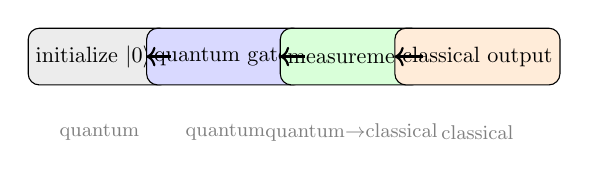
\begin{tikzpicture}[node distance=2cm, scale=0.8, every node/.style={scale=0.8}]
    \node[draw, rounded corners, fill=gray!15, minimum width=1.8cm, minimum height=0.9cm] (init) {initialize $\ket{0}^n$};
    \node[draw, rounded corners, fill=blue!15, minimum width=1.8cm, minimum height=0.9cm, right of=init] (gates) {quantum gates};
    \node[draw, rounded corners, fill=green!15, minimum width=1.8cm, minimum height=0.9cm, right of=gates] (meas) {measurement};
    \node[draw, rounded corners, fill=orange!15, minimum width=2cm, minimum height=0.9cm, right of=meas] (class) {classical output};

    \draw[->, thick] (init) -- (gates);
    \draw[->, thick] (gates) -- (meas);
    \draw[->, thick] (meas) -- (class);

    \node[below of=init, yshift=0.8cm, gray, font=\small] {quantum};
    \node[below of=gates, yshift=0.8cm, gray, font=\small] {quantum};
    \node[below of=meas, yshift=0.8cm, gray, font=\small] {quantum$\to$classical};
    \node[below of=class, yshift=0.8cm, gray, font=\small] {classical};
\end{tikzpicture}
\end{center}

quantum circuits r read left to right. each horizontal line is a qubit. gates r applied in the order they appear from left to right. time flows left to right.

\begin{center}
\begin{quantikz}
\lstick{$\ket{0}$} & \gate{H} & \ctrl{1} & \gate{R_z(\theta)} & \meter{} \\
\lstick{$\ket{0}$} & \qw & \targ{} & \gate{X} & \meter{}
\end{quantikz}
\end{center}

this circuit:
\begin{enumerate}
    \item starts with two qubits in $\ket{00}$
    \item applies H to qubit 0
    \item applies CNOT with qubit 0 as control, qubit 1 as target
    \item applies $R_z(\theta)$ to qubit 0 and X to qubit 1
    \item measures both qubits
\end{enumerate}

\subsection{Circuit Identities}

some useful identities for simplifying circuits:

\begin{itemize}
    \item $HXH = Z$ (conjugating X by H gives Z)
    \item $HZH = X$ (conjugating Z by H gives X)
    \item $HYH = -Y$
    \item $X = HZH$ (can replace X with H-Z-H)
    \item CNOT$_{12}$ = $(I \otimes H) \cdot$CZ$_{12} \cdot (I \otimes H)$
\end{itemize}

\begin{example}
the following two circuits r equivalent:

\begin{center}
\begin{quantikz}
& \ctrl{1} & \qw \\
& \targ{} & \qw
\end{quantikz}
$\quad = \quad$
\begin{quantikz}
& \qw & \ctrl{1} & \qw & \qw \\
& \gate{H} & \ctrl{-1} & \gate{H} & \qw
\end{quantikz}
\end{center}

bcs CNOT = $(I \otimes H) \cdot$ CZ $\cdot (I \otimes H)$ and CZ is symmetric.
\end{example}

%% ========================================================
\section{Measurement in Different Bases}
%% ========================================================

\subsection{Measuring in the X Basis}

to measure in the $\{\ket{+}, \ket{-}\}$ basis, apply H before measuring in the computational basis:

\begin{center}
\begin{quantikz}
\lstick{$\ket{\psi}$} & \gate{H} & \meter{}
\end{quantikz}
\end{center}

\begin{intuition}
applying H before measurement rotates the measurement basis. instead of projecting onto $\ket{0}$ and $\ket{1}$, u r effectively projecting onto $\ket{+}$ and $\ket{-}$. outcome 0 means the state was closer to $\ket{+}$, outcome 1 means closer to $\ket{-}$.
\end{intuition}

\begin{example}
measure $\ket{\psi} = \frac{1}{\sqrt{2}}(\ket{0} + \ket{1}) = \ket{+}$ in the X basis:

apply H: $H\ket{+} = \ket{0}$.

measure in computational basis: get $0$ with probability 1.

so measuring $\ket{+}$ in the X basis always gives outcome ``$+$''. makes sense.
\end{example}

\subsection{Measuring in the Y Basis}

to measure in the Y basis $\{\ket{+i}, \ket{-i}\}$, apply $S^\dagger H$ before measuring:

\begin{center}
\begin{quantikz}
\lstick{$\ket{\psi}$} & \gate{S^\dagger} & \gate{H} & \meter{}
\end{quantikz}
\end{center}

\subsection{General Measurement Basis}

to measure in any orthonormal basis $\{\ket{b_0}, \ket{b_1}\}$, find the unitary $U$ that maps $\ket{b_i} \to \ket{i}$, apply $U$, and measure in the computational basis.

%% ========================================================
\section{The No-Cloning Theorem}
%% ========================================================

\begin{definition}
the \textbf{no-cloning theorem} states that there is no quantum operation that can copy an arbitrary unknown quantum state:
\[
\nexists \; U \text{ such that } U\ket{\psi}\ket{0} = \ket{\psi}\ket{\psi} \text{ for all } \ket{\psi}
\]
\end{definition}

\textbf{proof}: suppose such a $U$ exists. then for any two states $\ket{\phi}$ and $\ket{\psi}$:
\begin{align}
U\ket{\phi}\ket{0} &= \ket{\phi}\ket{\phi} \\
U\ket{\psi}\ket{0} &= \ket{\psi}\ket{\psi}
\end{align}

take the inner product of both sides:
\[
\braket{\phi|\psi}\braket{0|0} = \braket{\phi|\psi}\braket{\phi|\psi}
\]
\[
\braket{\phi|\psi} = \braket{\phi|\psi}^2
\]

this equation has only two solutions: $\braket{\phi|\psi} = 0$ or $\braket{\phi|\psi} = 1$. meaning either the states r identical or orthogonal. u cant clone arbitrary states --- contradiction. $\square$

\begin{keypoint}
no-cloning has huge implications:
\begin{itemize}
    \item u cant copy quantum information --- this is why quantum error correction is fundamentally different from classical error correction (cant just duplicate the data)
    \item u cant measure a state without disturbing it --- bcs measurement ``collapses'' the state
    \item quantum cryptography (QKD) works bcs eavesdroppers cant copy quantum signals without being detected
    \item in QML, u cant simply ``look at'' intermediate quantum states during computation without affecting the result
\end{itemize}
\end{keypoint}

%% ========================================================
\section{Entanglement}
%% ========================================================

\subsection{What Entanglement Actually Is}

we introduced entanglement in lecture 1 using the tensor product factorization test. now lets go deeper.

\begin{definition}
a pure state $\ket{\psi_{AB}}$ of a bipartite system is \textbf{entangled} if it cannot be written as a product state $\ket{a} \otimes \ket{b}$. equivalently, a state is entangled iff the reduced density matrix of either subsystem is mixed (has purity $< 1$).
\end{definition}

\begin{intuition}
entanglement means the whole system has more information than the sum of its parts. if u know everything abt the global state (its pure), but the local states r mixed (uncertain), then the information is encoded in \textbf{correlations} between the subsystems. these correlations r stronger than any classical correlations can be --- thats the essence of entanglement.
\end{intuition}

\begin{center}
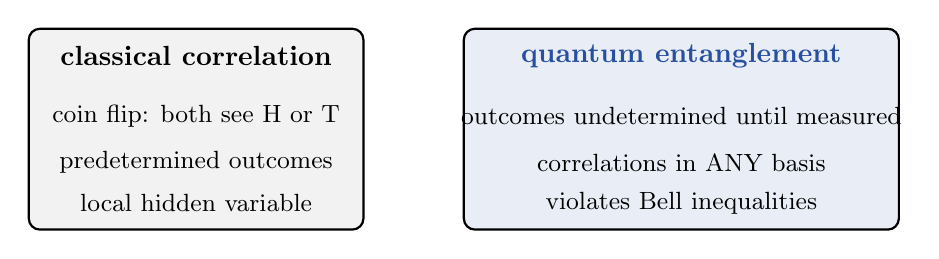
\begin{tikzpicture}[scale=0.85]
    % classical correlations
    \draw[thick, rounded corners, fill=gray!10] (-0.5, -0.5) rectangle (4.5, 2.5);
    \node[font=\bfseries] at (2, 2.1) {classical correlation};
    \node at (2, 1.2) {\small coin flip: both see H or T};
    \node at (2, 0.5) {\small predetermined outcomes};
    \node at (2, -0.1) {\small local hidden variable};

    % quantum entanglement
    \draw[thick, rounded corners, fill=circuitblue!10] (6, -0.5) rectangle (12.5, 2.5);
    \node[font=\bfseries, circuitblue] at (9.25, 2.1) {quantum entanglement};
    \node at (9.25, 1.2) {\small outcomes undetermined until measured};
    \node at (9.25, 0.5) {\small correlations in ANY basis};
    \node at (9.25, -0.1) {\small violates Bell inequalities};
\end{tikzpicture}
\end{center}

\subsection{Bell States}

the four bell states r the maximally entangled two-qubit states:

\begin{align}
\ket{\Phi^+} &= \frac{1}{\sqrt{2}}(\ket{00} + \ket{11}) \\
\ket{\Phi^-} &= \frac{1}{\sqrt{2}}(\ket{00} - \ket{11}) \\
\ket{\Psi^+} &= \frac{1}{\sqrt{2}}(\ket{01} + \ket{10}) \\
\ket{\Psi^-} &= \frac{1}{\sqrt{2}}(\ket{01} - \ket{10})
\end{align}

circuits to create all four bell states from $\ket{00}$:

\begin{center}
\begin{quantikz}
\lstick{$\ket{0}$} & \gate{H} & \ctrl{1} & \rstick{$\ket{\Phi^+}$} \qw \\
\lstick{$\ket{0}$} & \qw & \targ{} & \qw
\end{quantikz}
\hspace{0.5cm}
\begin{quantikz}
\lstick{$\ket{0}$} & \gate{X} & \gate{H} & \ctrl{1} & \rstick{$\ket{\Phi^-}$} \qw \\
\lstick{$\ket{0}$} & \qw & \qw & \targ{} & \qw
\end{quantikz}
\end{center}

\begin{center}
\begin{quantikz}
\lstick{$\ket{0}$} & \gate{H} & \ctrl{1} & \rstick{$\ket{\Psi^+}$} \qw \\
\lstick{$\ket{0}$} & \gate{X} & \targ{} & \qw
\end{quantikz}
\hspace{0.5cm}
\begin{quantikz}
\lstick{$\ket{0}$} & \gate{X} & \gate{H} & \ctrl{1} & \rstick{$\ket{\Psi^-}$} \qw \\
\lstick{$\ket{0}$} & \gate{X} & \qw & \targ{} & \qw
\end{quantikz}
\end{center}

\subsection{GHZ States}

\begin{definition}
the \textbf{GHZ state} for $n$ qubits:
\[
\ket{GHZ_n} = \frac{1}{\sqrt{2}}(\ket{0}^{\otimes n} + \ket{1}^{\otimes n})
\]
\end{definition}

circuit for 3-qubit GHZ:

\begin{center}
\begin{quantikz}
\lstick{$\ket{0}$} & \gate{H} & \ctrl{1} & \qw & \qw \\
\lstick{$\ket{0}$} & \qw & \targ{} & \ctrl{1} & \qw \\
\lstick{$\ket{0}$} & \qw & \qw & \targ{} & \qw
\end{quantikz}
\end{center}

step by step:
\begin{align}
\ket{000} &\xrightarrow{H_1} \frac{1}{\sqrt{2}}(\ket{0} + \ket{1})\ket{00} = \frac{1}{\sqrt{2}}(\ket{000} + \ket{100}) \\
&\xrightarrow{\text{CNOT}_{12}} \frac{1}{\sqrt{2}}(\ket{000} + \ket{110}) \\
&\xrightarrow{\text{CNOT}_{23}} \frac{1}{\sqrt{2}}(\ket{000} + \ket{111}) = \ket{GHZ_3}
\end{align}

\subsection{Quantifying Entanglement}

for pure bipartite states, entanglement can be measured using the \textbf{von Neumann entropy} of the reduced density matrix:

\[
\boxed{S(\rho_A) = -\text{tr}(\rho_A \log_2 \rho_A) = -\sum_i \lambda_i \log_2 \lambda_i}
\]

where $\lambda_i$ r the eigenvalues of $\rho_A$.

\begin{itemize}
    \item $S = 0$: product state (no entanglement)
    \item $S = 1$: maximally entangled (for two qubits)
    \item $0 < S < 1$: partially entangled
\end{itemize}

\begin{example}
for the bell state $\ket{\Phi^+}$, we showed $\rho_A = I/2$, which has eigenvalues $1/2, 1/2$:
\[
S = -\frac{1}{2}\log_2\frac{1}{2} - \frac{1}{2}\log_2\frac{1}{2} = -\frac{1}{2}(-1) - \frac{1}{2}(-1) = 1 \text{ ebit}
\]
maximally entangled, as expected.
\end{example}

%% ========================================================
\section{Quantum Teleportation}
%% ========================================================

quantum teleportation is one of the most beautiful protocols in quantum information. it allows u to transmit an unknown quantum state using only classical communication and a pre-shared entangled pair.

heres the high-level protocol as a flowchart:

\begin{center}
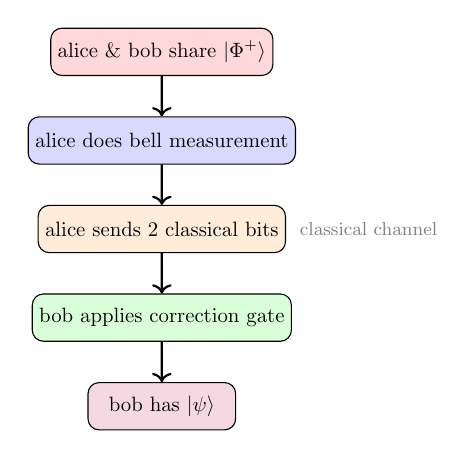
\begin{tikzpicture}[node distance=1.5cm, scale=0.75, every node/.style={scale=0.75}]
    \node[draw, rounded corners, fill=red!15, minimum width=2.5cm, minimum height=0.8cm] (share) {alice \& bob share $\ket{\Phi^+}$};
    \node[draw, rounded corners, fill=blue!15, minimum width=2.5cm, minimum height=0.8cm, below of=share] (bell) {alice does bell measurement};
    \node[draw, rounded corners, fill=orange!15, minimum width=2.5cm, minimum height=0.8cm, below of=bell] (send) {alice sends 2 classical bits};
    \node[draw, rounded corners, fill=green!15, minimum width=2.5cm, minimum height=0.8cm, below of=send] (fix) {bob applies correction gate};
    \node[draw, rounded corners, fill=purple!15, minimum width=2.5cm, minimum height=0.8cm, below of=fix] (done) {bob has $\ket{\psi}$};

    \draw[->, thick] (share) -- (bell);
    \draw[->, thick] (bell) -- (send);
    \draw[->, thick] (send) -- (fix);
    \draw[->, thick] (fix) -- (done);

    \node[right of=send, xshift=2cm, gray, font=\small] {classical channel};
\end{tikzpicture}
\end{center}

\subsection{Setup}

alice has an unknown qubit $\ket{\psi} = \alpha\ket{0} + \beta\ket{1}$ that she wants to send to bob. they share a bell pair $\ket{\Phi^+}$.

total initial state (3 qubits: alice's data qubit, alice's half of bell pair, bob's half of bell pair):
\[
\ket{\psi}_1 \otimes \ket{\Phi^+}_{23} = (\alpha\ket{0} + \beta\ket{1}) \otimes \frac{1}{\sqrt{2}}(\ket{00} + \ket{11})
\]

\subsection{The Protocol}

\begin{center}
\begin{quantikz}
\lstick{$\ket{\psi}$} & \ctrl{1} & \gate{H} & \meter{} & \cwbend{2} \\
\lstick{$\ket{\Phi^+}$} & \targ{} & \qw & \meter{} & \cwbend{1} \\
& \qw & \qw & \qw & \gate{X^{m_2}Z^{m_1}} & \rstick{$\ket{\psi}$} \qw
\end{quantikz}
\end{center}

\subsection{Step-by-Step Walkthrough}

expand the initial state:
\[
\frac{1}{\sqrt{2}}[\alpha\ket{0}(\ket{00} + \ket{11}) + \beta\ket{1}(\ket{00} + \ket{11})]
\]
\[
= \frac{1}{\sqrt{2}}[\alpha\ket{000} + \alpha\ket{011} + \beta\ket{100} + \beta\ket{111}]
\]

\textbf{step 1: CNOT on qubits 1,2:}
\[
\frac{1}{\sqrt{2}}[\alpha\ket{000} + \alpha\ket{011} + \beta\ket{110} + \beta\ket{101}]
\]

\textbf{step 2: H on qubit 1:}

using $H\ket{0} = \frac{1}{\sqrt{2}}(\ket{0}+\ket{1})$ and $H\ket{1} = \frac{1}{\sqrt{2}}(\ket{0}-\ket{1})$:

\begin{align}
&\frac{1}{2}[\alpha(\ket{0}+\ket{1})\ket{00} + \alpha(\ket{0}+\ket{1})\ket{11} + \beta(\ket{0}-\ket{1})\ket{10} + \beta(\ket{0}-\ket{1})\ket{01}]
\end{align}

regroup by alice's measurement outcomes (first two qubits):
\begin{align}
= \frac{1}{2}[&\ket{00}(\alpha\ket{0} + \beta\ket{1}) + \ket{01}(\alpha\ket{1} + \beta\ket{0}) \\
+ &\ket{10}(\alpha\ket{0} - \beta\ket{1}) + \ket{11}(\alpha\ket{1} - \beta\ket{0})]
\end{align}

\textbf{step 3: alice measures} qubits 1 and 2, gets one of four outcomes with equal probability $1/4$:

\begin{center}
\begin{tabular}{c|c|c}
alice measures & bob's state & correction \\
\hline
$\ket{00}$ & $\alpha\ket{0} + \beta\ket{1} = \ket{\psi}$ & none ($I$) \\
$\ket{01}$ & $\alpha\ket{1} + \beta\ket{0} = X\ket{\psi}$ & apply $X$ \\
$\ket{10}$ & $\alpha\ket{0} - \beta\ket{1} = Z\ket{\psi}$ & apply $Z$ \\
$\ket{11}$ & $\alpha\ket{1} - \beta\ket{0} = ZX\ket{\psi}$ & apply $ZX$ \\
\end{tabular}
\end{center}

\textbf{step 4:} alice sends her 2 classical bits to bob. bob applies the corresponding correction. result: bob has $\ket{\psi}$.

\begin{keypoint}
teleportation doesnt violate no-cloning or special relativity:
\begin{itemize}
    \item alice's original state is destroyed (no cloning) --- after measurement, her qubits r in a definite state $\ket{m_1 m_2}$, not $\ket{\psi}$
    \item bob needs alice's classical bits to reconstruct the state (no FTL communication) --- without the correction, bob's qubit looks maximally mixed
    \item the state is ``teleported'' not ``transmitted'' --- no physical qubit travels from alice to bob
\end{itemize}
\end{keypoint}

\begin{intuition}
teleportation is a resource conversion protocol. it converts 1 ebit of entanglement + 2 classical bits into 1 qubit of quantum communication. the entanglement acts as a ``quantum channel'' that was established beforehand.
\end{intuition}

%% ========================================================
\section{Superdense Coding}
%% ========================================================

superdense coding is the ``reverse'' of teleportation. instead of sending a quantum state using classical communication + entanglement, u send 2 classical bits by transmitting only 1 qubit (plus using 1 ebit of pre-shared entanglement).

\subsection{The Protocol}

alice and bob share a bell pair $\ket{\Phi^+} = \frac{1}{\sqrt{2}}(\ket{00} + \ket{11})$.

alice wants to send 2 classical bits $m_1 m_2$ to bob. she applies a gate to her qubit based on the message:

\begin{center}
\begin{tabular}{c|c|c}
message & alice applies & resulting state \\
\hline
00 & $I$ & $\ket{\Phi^+} = \frac{1}{\sqrt{2}}(\ket{00} + \ket{11})$ \\
01 & $X$ & $\ket{\Psi^+} = \frac{1}{\sqrt{2}}(\ket{10} + \ket{01})$ \\
10 & $Z$ & $\ket{\Phi^-} = \frac{1}{\sqrt{2}}(\ket{00} - \ket{11})$ \\
11 & $ZX$ & $\ket{\Psi^-} = \frac{1}{\sqrt{2}}(\ket{10} - \ket{01})$ \\
\end{tabular}
\end{center}

alice sends her qubit to bob. now bob has both qubits of a bell state. he performs a bell measurement (CNOT then H, then measure) to determine which bell state it is, recovering the 2-bit message.

\begin{center}
\begin{quantikz}
\lstick{alice's qubit} & \gate{U_{m_1m_2}} & \qw & \qw & \ctrl{1} & \gate{H} & \meter{} \\
\lstick{bob's qubit} & \qw & \qw & \qw & \targ{} & \qw & \meter{}
\end{quantikz}
\end{center}

\subsection{Bell Measurement}

the key circuit for distinguishing bell states:

\begin{center}
\begin{quantikz}
& \ctrl{1} & \gate{H} & \meter{} \\
& \targ{} & \qw & \meter{}
\end{quantikz}
\end{center}

this maps:
\begin{align}
\ket{\Phi^+} &\to \ket{00} \\
\ket{\Psi^+} &\to \ket{01} \\
\ket{\Phi^-} &\to \ket{10} \\
\ket{\Psi^-} &\to \ket{11}
\end{align}

\begin{example}
verify for $\ket{\Phi^+} = \frac{1}{\sqrt{2}}(\ket{00} + \ket{11})$:

CNOT: $\frac{1}{\sqrt{2}}(\ket{00} + \ket{10}) = \frac{1}{\sqrt{2}}(\ket{0} + \ket{1})\ket{0} = \ket{+}\ket{0}$

H on first qubit: $H\ket{+} = \ket{0}$

final state: $\ket{00}$. measurement gives 00.
\end{example}

\begin{keypoint}
comparison of teleportation and superdense coding:
\begin{center}
\begin{tabular}{l|c|c}
 & teleportation & superdense coding \\
\hline
input & 1 qubit & 2 classical bits \\
resource & 1 ebit + 2 cbits & 1 ebit + 1 qubit \\
output & 1 qubit (at bob) & 2 classical bits (at bob) \\
\end{tabular}
\end{center}
they r ``dual'' protocols --- one converts ebits + cbits into qubits, the other converts ebits + qubits into cbits.
\end{keypoint}

%% ========================================================
\section{Important Quantum Circuit Patterns}
%% ========================================================

\subsection{Uniform Superposition}

to create an equal superposition over all $n$-qubit basis states:

\begin{center}
\begin{quantikz}
\lstick{$\ket{0}$} & \gate{H} & \qw \\
\lstick{$\ket{0}$} & \gate{H} & \qw \\
\lstick{$\ket{0}$} & \gate{H} & \qw \\
& \vdots & \\
\lstick{$\ket{0}$} & \gate{H} & \qw
\end{quantikz}
\end{center}

\[
H^{\otimes n}\ket{0}^{\otimes n} = \frac{1}{\sqrt{2^n}}\sum_{x=0}^{2^n-1}\ket{x}
\]

this creates a uniform superposition over all $2^n$ computational basis states using just $n$ hadamard gates. its the starting point for many quantum algorithms.

\subsection{Phase Kickback}

\begin{keypoint}
\textbf{phase kickback} is a crucial phenomenon where a controlled-U gate ``kicks back'' the eigenvalue phase onto the control qubit.

if $U\ket{u} = e^{i\phi}\ket{u}$ (i.e., $\ket{u}$ is an eigenstate of $U$ with eigenvalue $e^{i\phi}$), then:
\[
\text{C-}U \ket{+}\ket{u} = \frac{1}{\sqrt{2}}(\ket{0}\ket{u} + e^{i\phi}\ket{1}\ket{u}) = \frac{1}{\sqrt{2}}(\ket{0} + e^{i\phi}\ket{1})\ket{u}
\]

the phase $e^{i\phi}$ appears on the \textbf{control} qubit, not the target. the target is unchanged.
\end{keypoint}

phase kickback is the mechanism behind:
\begin{itemize}
    \item the deutsch-jozsa algorithm
    \item quantum phase estimation
    \item grover's diffusion operator
    \item many other quantum algorithms
\end{itemize}

\begin{example}
phase kickback with the Z gate. since $Z\ket{1} = -\ket{1}$ ($\ket{1}$ is an eigenstate of Z with eigenvalue $-1$):

\begin{center}
\begin{quantikz}
\lstick{$\ket{+}$} & \ctrl{1} & \rstick{$\ket{-}$} \qw \\
\lstick{$\ket{1}$} & \gate{Z} & \rstick{$\ket{1}$} \qw
\end{quantikz}
\end{center}

the control qubit picks up the phase: $\ket{+} \to \frac{1}{\sqrt{2}}(\ket{0} + (-1)\ket{1}) = \ket{-}$.

the target stays as $\ket{1}$.
\end{example}

%% ========================================================
\section{Summary}
%% ========================================================

\begin{keypoint}
wt we covered:
\begin{enumerate}
    \item \textbf{single qubit gates}: pauli gates (X, Y, Z), hadamard (H), phase gates (S, T), rotation gates ($R_x$, $R_y$, $R_z$)
    \item \textbf{multi-qubit gates}: CNOT, CZ, toffoli, SWAP
    \item \textbf{universal gate sets}: $\{H, T, \text{CNOT}\}$ is enough for any quantum computation
    \item \textbf{circuit model}: circuits r read left to right, gates r matrices, composition is matrix multiplication
    \item \textbf{measurement}: can measure in any basis by applying a basis-changing unitary first
    \item \textbf{no-cloning}: u cant copy unknown quantum states --- fundamental constraint
    \item \textbf{entanglement}: bell states, GHZ states, quantified by von neumann entropy
    \item \textbf{teleportation}: send a qubit using 1 ebit + 2 cbits
    \item \textbf{superdense coding}: send 2 cbits using 1 ebit + 1 qubit
    \item \textbf{phase kickback}: eigenvalue phases ``kick back'' onto control qubits --- key mechanism for many algorithms
\end{enumerate}
these r the building blocks. every quantum algorithm, including QML algorithms, is built from these components.
\end{keypoint}

\end{document}
